\section{Structure}
    Every syllable is written as a single block built from up to three parts: an initial consonant $\mathrm{c}_i$, a total vowel $\mathrm{v}_t$, and a final optional consonant $\mathrm{c}_o$.
    
    \begin{figure}[H]
        \centering
        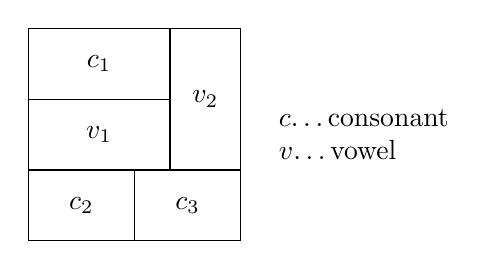
\begin{tikzpicture}[scale=0.9]
            \draw (0,2) rectangle (2,3) node[pos=.5] {$c_1$};
            \draw (0,1) rectangle (2,2) node[pos=.5] {$v_1$};
            \draw (2,1) rectangle (3,3) node[pos=.5] {$v_2$};
            \draw (0,0) rectangle (1.5,1) node[pos=.5] {$c_2$};
            \draw (1.5,0) rectangle (3,1) node[pos=.5] {$c_3$};
            \node[anchor=west, align=left] at (3.4,1.5) {$c$\ldots consonant\\ $v$\ldots vowel};
        \end{tikzpicture}
        \caption{Basic structure of a Hangul syllable block}
        \label{fig:block}
    \end{figure}

    \cref{fig:block} shows the block structure. Letters are read in this order:

    \begin{equation}
        \mathrm{Syllable} = 
        \underbrace{\mathrm{c}_1}_{\text{initial consonant}\ \mathrm{c}_i} + \underbrace{(\mathrm{v}_1 + \mathrm{v}_2)}_{\text{total vowel}\ \mathrm{v}_t} + \underbrace{(\mathrm{c}_2 + \mathrm{c}_3)}_{\text{optional consonant}\ \mathrm{c}_o}  \label{eq:syllable_structure}
    \end{equation}
    $\mathrm{c}_o$ \cref{eq:syllable_structure} If the optional consonant $\mathrm{c}_o$ uses both $\mathrm{c}_2$ and $\mathrm{c}_3$, then they are spoken together as a single consonant sound by compressing the sound of the individual consonants.